\section{Introduction}
The online video streaming is the most popular service from the Internet. With the introduction of the video streaming system over the HTTP and in build player in HTML5, make it easier to start a new video streaming service in one hand, on the other hand the pervasive penetration of the LTE network, make it easier for the smartphone user to watch the online video. On top HTTP and HTML5, dynamic adaptation of the audio video quality allows provider to make the service tolarent to frequent network change. Obviously, this technologies gain attention of researcher all around the globe. In this work, we discuss the technological advancement for video streaming using HTTP.

Online video streaming can be largly categorised in three categories: i) static video or video on demand (VoD) streaming, ii) live video streaming and iii) interactive video streaming. Video streaming services like YouTube, NetFlix, Prime videos are falls into the video on demand category. Here the videos are prerecorded and preproccessed. YouTube-Live, Periscope, Twitch provide live video streaming Category. The only difference between VoD and live video streaming is that in case of live streaming video the not preproccessed as it is not ready yet. The services like video conferencing, webinar are falls in third category, the interactive video. The interactive online videos are not only bidirectional, but also extremely delay sensitive. Unlike VoD or live streaming, it is okay for interactive video streaming drop several frames than stall for data. So, the technology requirement for the interactive video is very different in every aspect. In our work, we concentrated on the VoD and live video streaming over HTTP only.

HTTP is a widely acceptable protocol as it serve the World-Wide-Web (WWW). Most of the firewalls, proxies and NAT-boxes allow HTTP protocol. HTTPS, the secure version of HTTP is equally acceptable of the network administrator or different organisation. So, the HTTP(S) based video streaming services also allowed by those firewalls, proxies and NAT boxes. This one feature, favored HTTP(S) based video streaming over existing video streaming system.

On top of HTTP based video streaming system, service provider can now adapt video quality according to the available network quality. It reduce the rebuffering significantly. Currently most of the online video service support adaptive video streaming as it provide better quality of experience to the viewers. Techonologies like MPEG-DASH (dynamic adaptive streaming over HTTP), Apple's HLS, SmoothStream by Microsoft support dynamic adaptive streaming. Although this technologies are developed by different organizations, they works almost identically. In our work, we concentrate on the DASH only as it is mostly a guideline than a product and the a open source implementation of DASH is available.

DASH or DASH like video streaming system changes video quality on the fly running adaptive bitrate algorithm (ABR). Selection of ABR is crucial as the overall quality of experience dependent on this algorithm. It ABR algorithms job to provide minimal rebuffering while maintaining better video quality. In our survey we first discuss the details of DASH and different components of DASH. Then we disccus application of DASH in YouTube, a major video streaming provider and latest research on the ABR for providing better QoE for both VoD and live streaming in different scenerios.

\subsection{DASH}
\begin{figure}[!t]
	\centering
	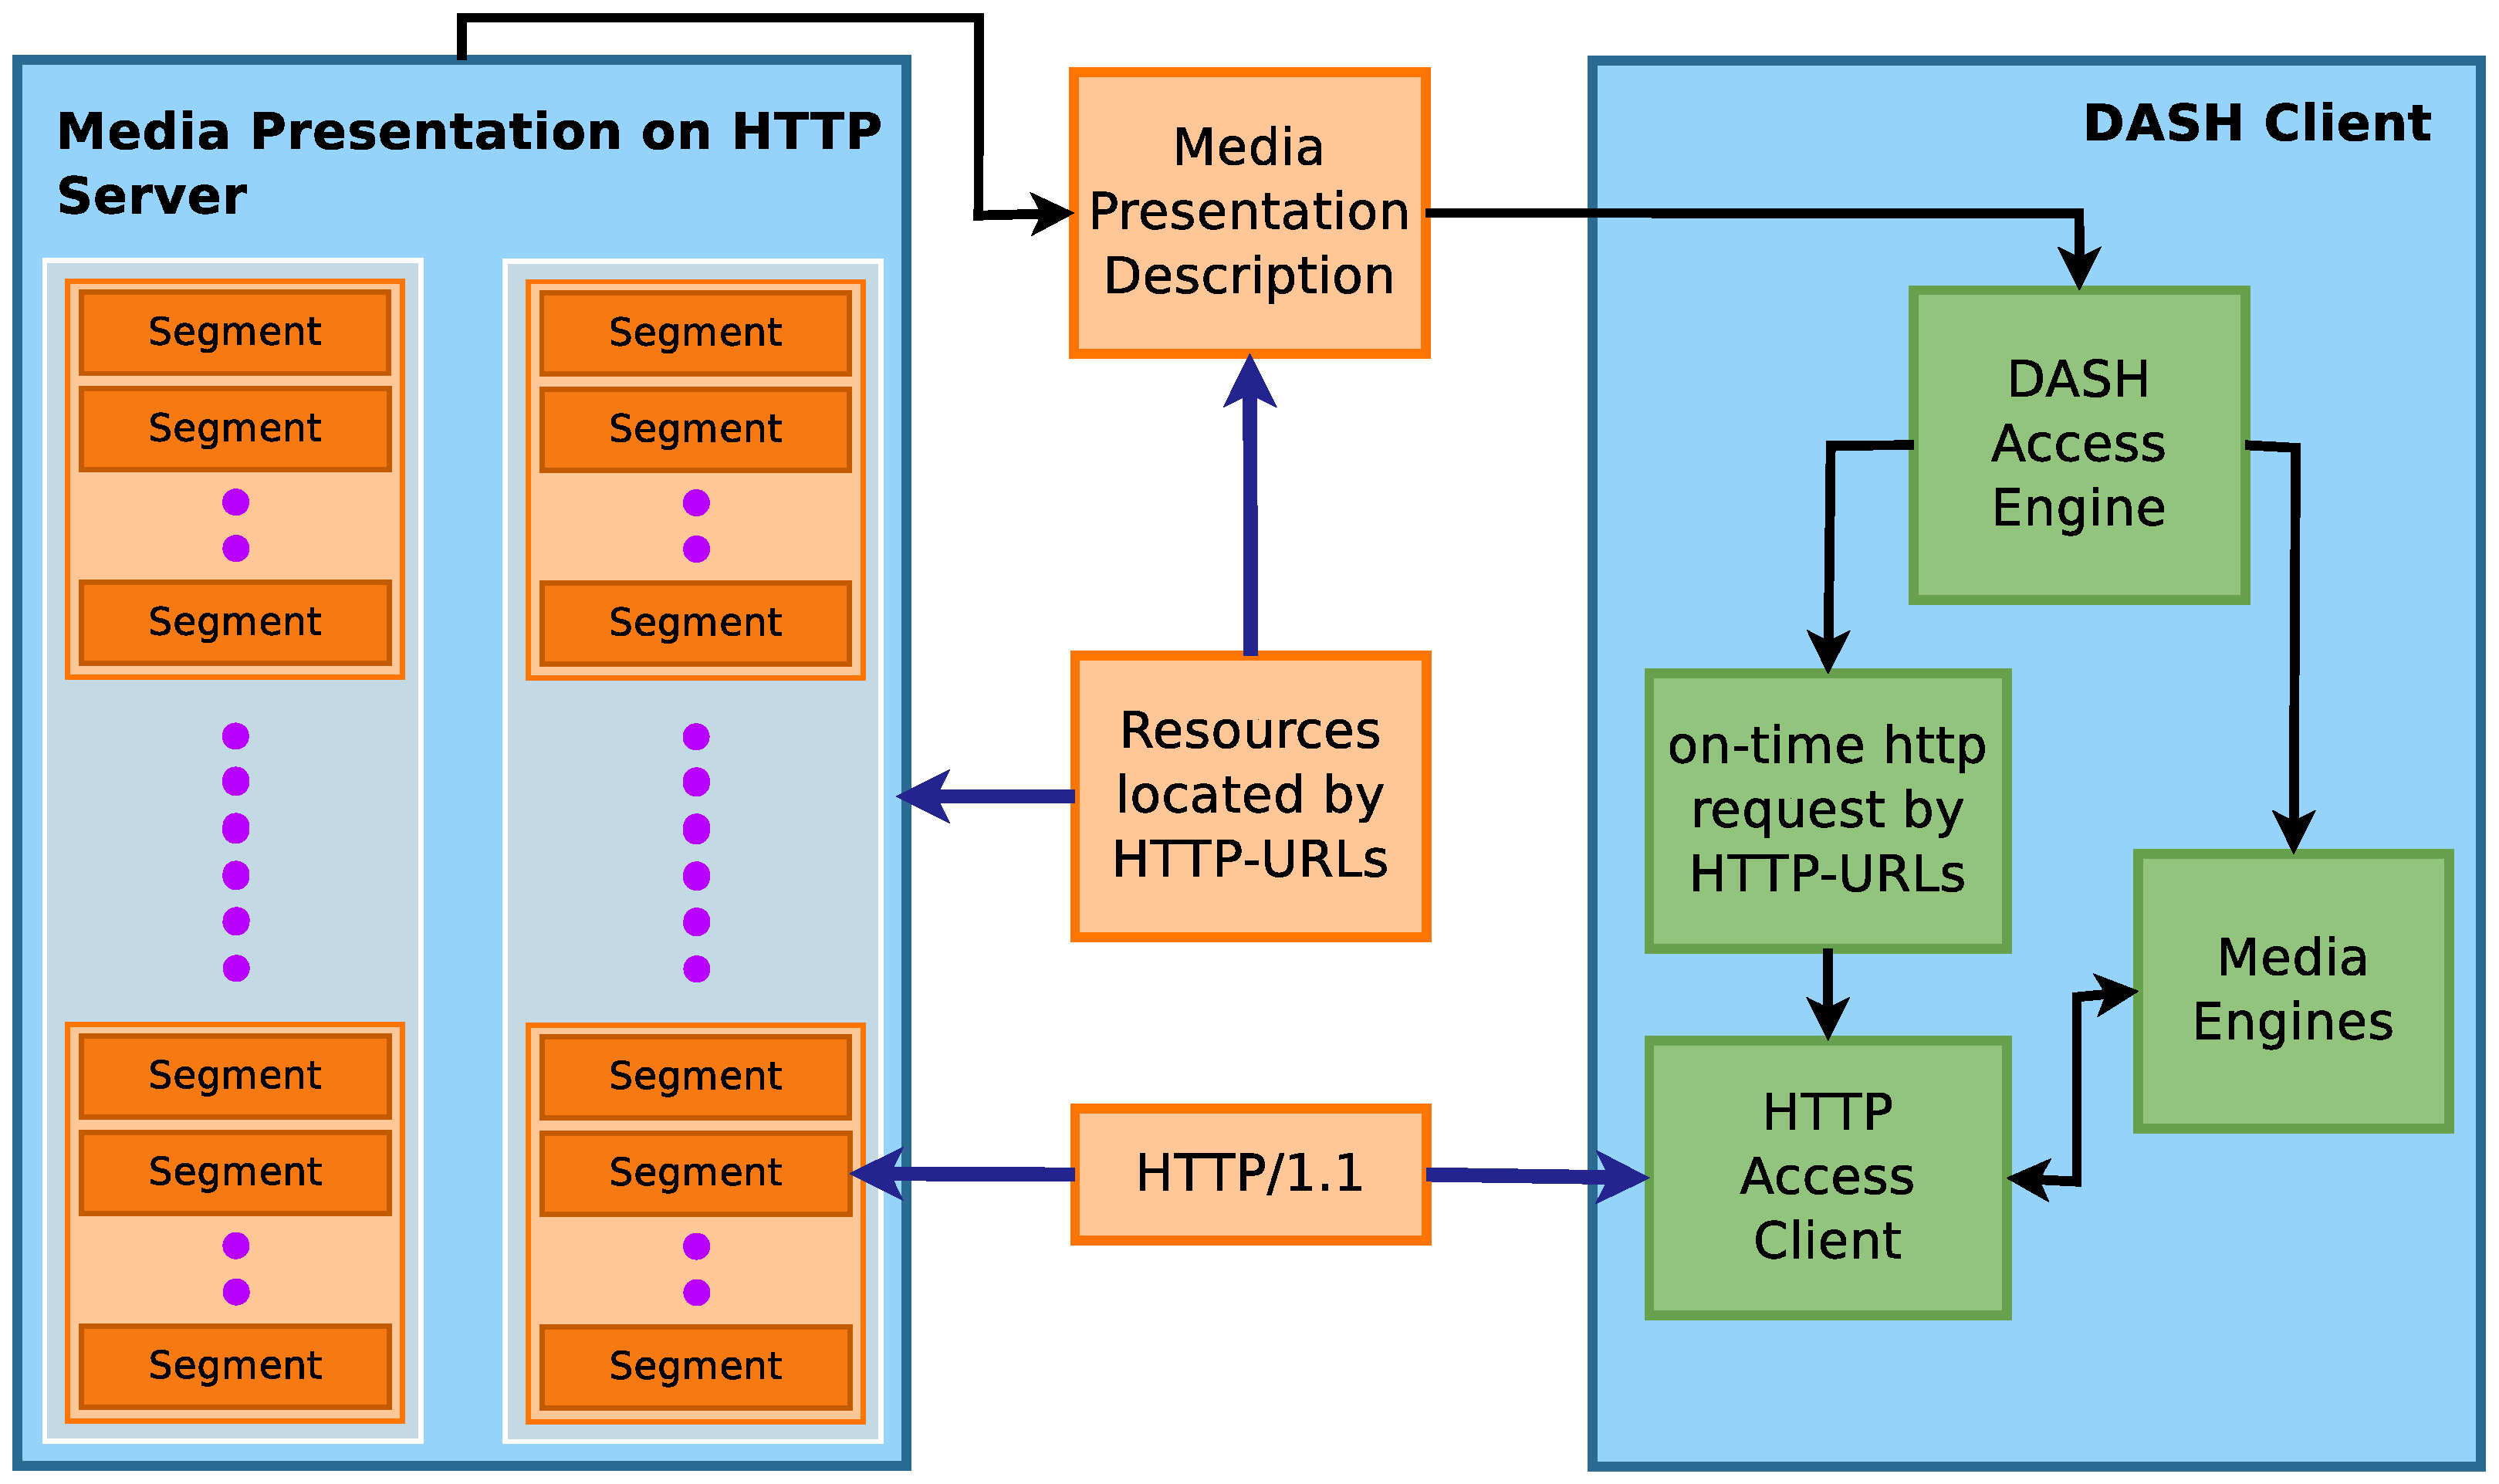
\includegraphics[scale=0.15]{img/dash-arch}
	\caption{\small{DASH Architecture -- On the left side, the server-side media storage is shown, where content is divided into small segments of alternative bit-rates. On the right side, the DASH client architecture is shown; the {\it DASH Access Engine} monitors network bandwidth at the client and accordingly decides which segment to request from the server. (Image Source: https://www.w3.org/2011/09/webtv/slides/W3C-Workshop.pdf)}}
	\label{fig:dash}
\end{figure}
%
Dynamic Adaptive Streaming over HTTP (DASH), also referred to as MPEG-DASH, is an adaptive bit-rate solution for video streaming, which enables client-operated video delivery over HTTP.
%
DASH is implemented by breaking down the video content into small segments, each worth a short duration of playback time.
%
For every segment of playback time, alternative versions at various bit-rates are available at the server.
%
The client typically requests for the highest quality segment possible under current network conditions, such that it is received (downloaded) in time for playback, without causing stalling or re-buffering. 
%
However, DASH is not a protocol -- it only specifies an architecture (Fig.~\ref{fig:dash}) to enable adaptive video streaming over HTTP.
%
Every video streaming service (e.g., YouTube, Netflix, etc.) is free to define its own implementation of the DASH modules.

\subsection{ABR}
Adaptive bitrate algorithm or ABR algorithm is the heart of the DASH. ABR decide when and which quality to download based on network quality and other parameter. Primary job of any ABR algorithm is improve user experience by selecting appropriate video quality for the a segment. As the online video streaming become one of the most popular service in the Internet, it become more prevalent to improve ABR algorithm to provide better QoE in different. The problem attract researcher from academic as well as the industries. Researcher start exploiting different areas of video streaming with a common goal, i.e. improving QoE for end user.

\subsection{QoE}
Quality of Experience is a important parameter in any field which involves end users. In case of the video streaming, QoE is metric to measure whether user have enjoyed the video or not. QoE is mostly a user perspective and it depends on several factor such as startup delay, quality flactuation, overall quality, rebuffering, audio/video device, video content. Although all this parameters are important, it is difficult to measure user dependent parameter and video content. Several researcher tried to to find best measurable metric to calculate QoE which can be acceptable. Mok \etal \cite{5990550} tried to calculate QoE from the network QoS. Infact they suggested that user QoS (or QoS of HTTP) is the QoE. 
